\documentclass[tikz,border=6pt]{standalone}

\usepackage[T1]{fontenc}
\usepackage{lmodern}
\usepackage{xcolor}
\usepackage{tikz}
\usetikzlibrary{positioning,calc,arrows.meta,shadows.blur}

\definecolor{navy}{RGB}{27,54,93}
\definecolor{blue}{RGB}{73,125,209}
\definecolor{lightblue}{RGB}{232,240,255}
\definecolor{midblue}{RGB}{208,223,250}
\definecolor{textdark}{RGB}{33,40,52}
\definecolor{lineblue}{RGB}{107,129,170}

\begin{document}
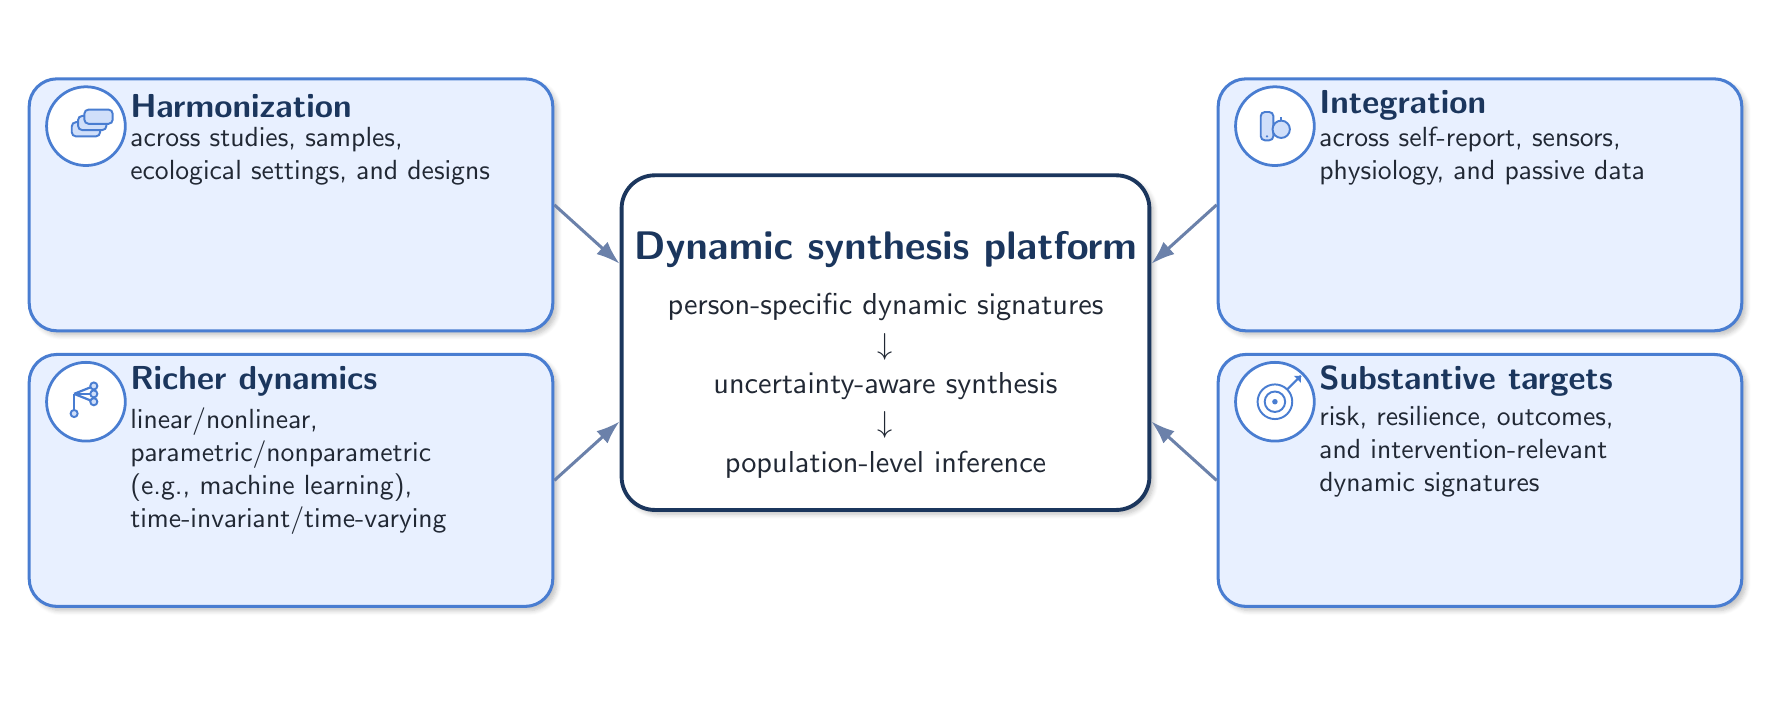
\begin{tikzpicture}[
		x=1cm,
		y=1cm,
		>=Latex,
		font=\sffamily,
		box/.style={
			rounded corners=10pt,
			draw=blue,
			line width=1.1pt,
			fill=lightblue,
			blur shadow={
				shadow blur steps=6,
				shadow xshift=1.5pt,
				shadow yshift=-1.5pt,
				shadow opacity=25
			},
			minimum width=6.65cm,
			minimum height=3.20cm,
			inner sep=0pt
		},
		core/.style={
			rounded corners=12pt,
			draw=navy,
			line width=1.4pt,
			fill=white,
			blur shadow={
				shadow blur steps=6,
				shadow xshift=1.5pt,
				shadow yshift=-1.5pt,
				shadow opacity=25
			},
			align=center,
			inner sep=10pt,
			minimum height=4.25cm,
			text width=6.0cm
		},
		iconcircle/.style={
			circle,
			draw=blue,
			line width=1pt,
			fill=white,
			minimum size=1.0cm,
			inner sep=0pt
		},
		arrow/.style={-{Latex[length=3mm,width=2.1mm]}, line width=1.1pt, draw=lineblue},
		smalltxt/.style={font=\sffamily\fontsize{10.2}{11.9}\selectfont, text=textdark},
		boxtitle/.style={font=\sffamily\bfseries\fontsize{12.9}{14.6}\selectfont, text=navy},
		coretitle/.style={font=\sffamily\bfseries\fontsize{14.7}{17}\selectfont, text=navy},
		coretxt/.style={font=\sffamily\fontsize{11.1}{13.4}\selectfont, text=textdark}
	]
	
	% Larger canvas
	\path[draw=none] (-1.8,0.9) rectangle (19.8,9.2);
	
	% Core
	\node[core] (core) at (9,5.2) {};
	\node[coretitle, align=center, text width=10cm] at ($(core.center)+(0,1.18)$) {Dynamic synthesis platform};
	\node[coretxt] at ($(core.center)+(0,0.45)$) {person-specific dynamic signatures};
	\node[coretxt] at ($(core.center)+(0,-0.05)$) {$\downarrow$};
	\node[coretxt] at ($(core.center)+(0,-0.55)$) {uncertainty-aware synthesis};
	\node[coretxt] at ($(core.center)+(0,-1.05)$) {$\downarrow$};
	\node[coretxt] at ($(core.center)+(0,-1.55)$) {population-level inference};
	
	% Outer boxes moved farther out
	\node[box] (harm) at (1.45,6.95) {};
	\node[box] (integrate) at (16.55,6.95) {};
	\node[box] (models) at (1.45,3.45) {};
	\node[box] (targets) at (16.55,3.45) {};
	
	% Icon circles
	\node[iconcircle] at ($(harm.north west)+(0.74,-0.62)$) (iharm) {};
	\node[iconcircle] at ($(integrate.north west)+(0.74,-0.62)$) (iint) {};
	\node[iconcircle] at ($(models.north west)+(0.74,-0.62)$) (imod) {};
	\node[iconcircle] at ($(targets.north west)+(0.74,-0.62)$) (itar) {};
	
	% Harmonization icon
	\foreach \i/\dx/\dy in {1/0/0,2/0.08/0.08,3/0.16/0.16}{
		\draw[draw=blue, fill=midblue, line width=0.7pt, rounded corners=1.5pt]
		($(iharm.center)+(-0.18+\dx,-0.13+\dy)$) rectangle
		($(iharm.center)+(0.18+\dx,0.05+\dy)$);
	}
	
	% Integration icon
	\draw[draw=blue, fill=midblue, line width=0.7pt, rounded corners=1.5pt]
	($(iint.center)+(-0.18,-0.18)$) rectangle ($(iint.center)+(-0.02,0.18)$);
	\fill[blue] ($(iint.center)+(-0.10,-0.13)$) circle (0.016);
	\draw[draw=blue, fill=midblue, line width=0.7pt]
	($(iint.center)+(0.08,-0.04)$) circle (0.11);
	\draw[blue, line width=0.7pt] ($(iint.center)+(-0.02,0)$) -- ($(iint.center)+(-0.03,0)$);
	\draw[blue, line width=0.7pt] ($(iint.center)+(0.08,0.07)$) -- ($(iint.center)+(0.08,0.12)$);
	
	% Models icon
	\draw[blue, line width=0.8pt] ($(imod.center)+(-0.15,-0.15)$) -- ($(imod.center)+(-0.15,0.10)$);
	\draw[blue, line width=0.8pt] ($(imod.center)+(-0.15,0.10)$) -- ($(imod.center)+(0.10,0.20)$);
	\draw[blue, line width=0.8pt] ($(imod.center)+(-0.15,0.10)$) -- ($(imod.center)+(0.10,0.10)$);
	\draw[blue, line width=0.8pt] ($(imod.center)+(-0.15,0.10)$) -- ($(imod.center)+(0.10,0.00)$);
	\foreach \dx/\dy in {-0.15/-0.15,0.10/0.20,0.10/0.10,0.10/0.00}{
		\filldraw[fill=midblue, draw=blue, line width=0.7pt]
		([shift={(\dx,\dy)}]imod.center) circle (0.045);
	}
	
	% Targets icon
	\draw[blue, line width=0.7pt] (itar.center) circle (0.22);
	\draw[blue, line width=0.7pt] (itar.center) circle (0.13);
	\fill[blue] (itar.center) circle (0.035);
	\draw[blue, line width=0.8pt] ($(itar.center)+(0.16,0.16)$) -- ($(itar.center)+(0.33,0.33)$);
	\fill[blue] ($(itar.center)+(0.33,0.33)$) --
	($(itar.center)+(0.24,0.33)$) --
	($(itar.center)+(0.33,0.24)$) -- cycle;
	
	% Box text
	\node[boxtitle, anchor=west, align=left]
	at ($(harm.north west)+(1.18,-0.36)$) {Harmonization};
	\node[smalltxt, anchor=west, align=left]
	at ($(harm.north west)+(1.18,-1.00)$)
	{across studies, samples,\\ecological settings, and designs};
	
	\node[boxtitle, anchor=west, align=left]
	at ($(integrate.north west)+(1.18,-0.36)$) {Integration};
	\node[smalltxt, anchor=west, align=left]
	at ($(integrate.north west)+(1.18,-1.00)$)
	{across self-report, sensors,\\physiology, and passive data};
	
	\node[boxtitle, anchor=west, align=left]
	at ($(models.north west)+(1.18,-0.36)$) {Richer dynamics};
	\node[smalltxt, anchor=west, align=left]
	at ($(models.north west)+(1.18,-1.50)$)
	{linear/nonlinear,\\parametric/nonparametric\\(e.g., machine learning),\\time-invariant/time-varying};
	
	\node[boxtitle, anchor=west, align=left]
	at ($(targets.north west)+(1.18,-0.36)$) {Substantive targets};
	\node[smalltxt, anchor=west, align=left]
	at ($(targets.north west)+(1.18,-1.25)$)
	{risk, resilience, outcomes,\\and intervention-relevant\\dynamic signatures};
	
	% Arrows
	\draw[arrow] (harm.east) -- ($(core.west)+(0,1.0)$);
	\draw[arrow] (integrate.west) -- ($(core.east)+(0,1.0)$);
	\draw[arrow] (models.east) -- ($(core.west)+(0,-1.0)$);
	\draw[arrow] (targets.west) -- ($(core.east)+(0,-1.0)$);
	
\end{tikzpicture}
\end{document}
